\begin{frame}[allowframebreaks]{Dimensionality Reduction}

Autoencoders help us reduce the number of features in our data, similar to PCA, but in a more flexible way.

\begin{itemize}
    \item The encoder takes big, complex data and squeezes it into a smaller, simpler form.
    \item This smaller version keeps the important information.
    \item Great for making it easier to see patterns or to prepare data for other machine learning tasks.
\end{itemize}

\textbf{Example}: We can use autoencoders to turn images (like MNIST digits) into just 2 or 3 numbers, so we can plot and explore them easily.

\framebreak

\begin{figure}
    \centering
    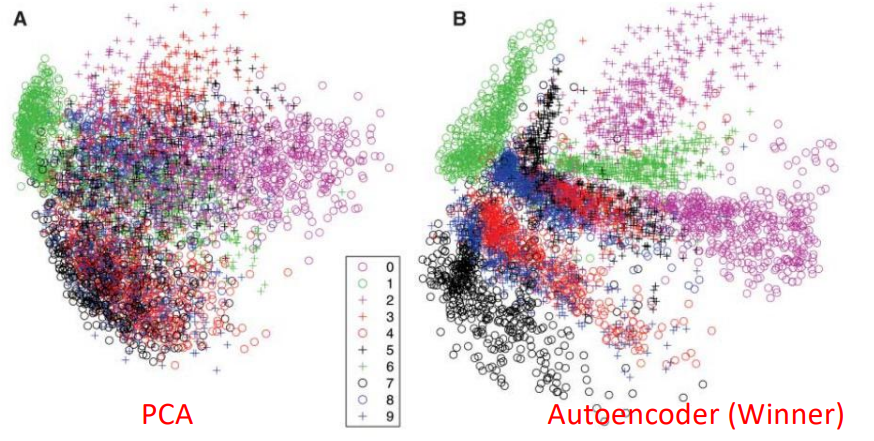
\includegraphics[height=0.75\textheight, width=\textwidth, keepaspectratio]{images/autoencoders/image_representation.PNG}
    \caption*{t-SNE visualization on MNIST digits dataset. PCA vs. Autoencoders. The image vector is projected into $\mathbb{R}^2$.}
\end{figure}

\end{frame}